\chapter{Path Integrals and Feynman--Kac formulae}

\label{ch:feynman_kac}

The imaginary-time path integral is closely connected with other ways of describing stochastic processes, 
such as stochastic differential equations and Fokker-Planck equations.
If stochastic paths are sampled from the path integral, then the path's evolution is governed by stochastic
differential equations or Langevin equations, where the noise is associated with the random sampling.
The path integral is also the solution to the diffusion or Fokker-Planck equation~\cite{Karatzas1991, Durrett1996}.
While stochastic differential equations describe single trajectories, the Fokker-Planck equation gives
the equation of motion for the ensemble-averaged probability distribution for the paths~\cite{Gardiner2009}.
The path integral solution to the diffusion equations is known as the Feynman--Kac formula,
after Feynman's work in describing the evolution of a quantum particle~\cite{Feynman1948},  and Kac's
work applying this to the diffusion equation~\cite{Kac1949}.

This chapter is devoted to deriving the Feynman--Kac formula with a source term.
We will develop analytical expressions for both TE and TM worldline path integrals 
in planar geometries.
These analytical formulae will be used in Ch.~\ref{ch:analytical} to demonstrate agreement 
with known results for both Casimir and Casimir--Polder energies.
The analytical expressions for ensemble-averaged path integrals are essential for handling the singular 
TM potential.  
In fact, these analytical results are necessary to even allow the TM numerics to proceed at all.
These analytical solutions are also useful in accelerating numerical methods relying 
on stochastic simulations.  

\section{Derivation of the Feynman--Kac formula }

In this section, we will derive the path integral as the solution to a diffusion equation,
using techniques from quantum mechanics.
The derivation will stay close in spirit to the one presented in Sakurai~\cite{Sakurai1994}, but it will
be extended to include a source term.%, as is more common for stochastic processes.
More formal derivations are available from mathematical~\cite{Cartier2004},
and probabilistic perspectives~\cite{Karatzas1991, Durrett1996}.  
A detailed discussion of the more formal probabilistic derivation is available in Steck \S 17.9~\cite{SteckNotes}.

The goal of this section is to find a solution $f(\vect{x},t)$ to the driven diffusion equation
\begin{equation}
  \partial_\tau f = \frac{1}{2}\nabla^2 f  - [V+\lambda]f +g,\label{eq:diffusion_equation}
\end{equation}
where the potential is given by $V=V(\vect{x})$, $\lambda$ is a constant, and the source term is $g=g(\vect{x},t)$.  
In this form $f$ corresponds to the probability distribution for a diffusing particle with a source
of particles $g$, which decays at a spatially dependent rate $V$.  
The Schr\"odinger equation is recovered under the $\tau\rightarrow -it$ substitution.
The differential equation can be written in operator form using the same Hilbert space 
conventions~(\ref{eq:commutation})--(\ref{eq:identity}) that were used for the worldline path integrals.
Note that $\hbar=1$ in this auxiliary Hilbert space.  
The diffusion equation~(\ref{eq:diffusion_equation}) can be written in operator form
\begin{equation}
  \partial_t\langle \vect{x}|f(t)\rangle = -\langle \vect{x}|
  \left(\frac{1}{2}\op{\vect{p}}^2 + V(\op{\vect{x}})+\lambda\right)|f(t)\rangle +\langle \vect{x}|g(t)\rangle.
  \label{eq:op_diffusion_eqn}
\end{equation}
This can be solved in analogy with solving the Schr\"odinger equation by introducing the evolution operator,
\begin{equation}
  U(t) := \exp\left[-\left(\frac{1}{2}\op{\vect{p}}^2 + V(\op{\vect{x}})+\lambda\right)t\right].
\end{equation}
Eq.~(\ref{eq:op_diffusion_eqn}) is written in the Schr\"odinger picture, where the operators are time 
independent, and the states $|f(t)\rangle$ carry all of the time dependence.  
After transforming to the Heisenberg picture where $|f(t)\rangle \rightarrow |\tilde{f}\rangle:=U^{-1}(t)|f(t)\rangle$,
the transformed vectors evolve in time according to
\begin{equation}
  \partial_t|\tilde{f}\rangle = U^{-1}(t)|g\rangle.
\end{equation}
This equation can be formally integrated with respect to time,
and after transforming back to the Schr\"odinger picture, the result is
\begin{equation}
  |f(t)\rangle = U(t)|f(0)\rangle + U(t) \int_0^t ds\, U(-s)|g(s)\rangle,
\end{equation}
where we used $U^{-1}(s)=U(-s)$.  
After combining the evolution operators, and projecting onto a final position $\vect{x}_N$ the solution is
\begin{equation}
  f(\vect{x}_N,t) = \langle \vect{x}_N|U(t)|f(0)\rangle + \int_0^t ds\, \langle \vect{x}_N|U(t-s)|g(s)\rangle.
  \label{eq:op_soln}
\end{equation}
The matrix elements in both terms have the same form $M = \langle \vect{x}_N|U(t)|f\rangle,$ so we will
develop the path integral for just one such matrix element.
For time-independent Hamiltonians, the evolution operator can be split into a product of $N$ identical evolution
operators $U(\Delta t)$ where  $\Delta t:=t/N$.
Position and momentum identities can be inserted between each term, with the result that
\begin{align}
  M
  = \int \prod_{k=0}^{N-1}\frac{d\vect{x}_{k}d\vect{p}_k}{(2\pi)^{D/2}}
  \prod_{j=1}^{N}\left(\langle \vect{x}_{k+1}| e^{-\op{H}\Delta t }|\vect{p}_k\rangle
    \langle \vect{p}_k| \vect{x}_{k}\rangle \right)
  \langle \vect{x}_0| f(0)\rangle.
\end{align}
The exponential operator is split into position and momentum pieces using the Baker-Campbell-Hausdorff theorem,
$ e^{-\Delta t [\op{p}^2+V(\op{x})]} = e^{-\Delta t V(\op{x})}e^{-\Delta t \op{p}^2} +\order(\Delta t^2)$.
The position and momentum operators then acquire the eigenvalues from operating to the left and right respectively,
\begin{align}
  M  = \int \prod_{k=0}^{N-1}\frac{d\vect{x}_{k}d\vect{p}_k}{(2\pi)^{D/2}}
  \prod_{j=1}^{N}\left( e^{-\vect{p}_k^2\Delta t/2 -[V(\vect{x}_{k+1})+\lambda]\Delta t+i\vect{p}_k\cdot(\vect{x}_{k+1}-\vect{x}_k)}\right)
  f(\vect{x}_0,0)
\end{align}
After carrying out the Gaussian momentum integrals, the matrix element is 
\begin{align}
  M %  &= \int \prod_{k=0}^{N-1}\frac{d\vect{x}_{k}d\vect{p}_k}{(2\pi)^{D}}
  % \prod_{j=1}^{N} e^{-\Delta t\left[\vect{p}_k^2/2 + V(\vect{x}_k,t_k)\right]+i\vect{p}_k\cdot(\vect{x}_{k+1}-\vect{x}_k)}
  % f(\vect{x}_0,0)\\
&= \int \prod_{k=0}^{N-1}d\vect{x}_{k}
  \prod_{j=1}^{N} \frac{e^{-(\vect{x}_{k+1}-\vect{x}_k)^2/(2\Delta t)}}{(2\pi\Delta t)^{D/2}}e^{- [V(\vect{x}_k)+\lambda]\Delta t}f(\vect{x}_0,0).
\end{align}
This is the traditional discrete form of the imaginary-time path integral.
We can make the connection to Brownian motion even clearer by changing integration variables.
The arguments of the Gaussians $\vect{x}_{k+1}-\vect{x}_{k}$ are zero mean random variables, with
variance $\Delta t$.  The Gaussians  can be interpreted as the probability distributions for the  vector Wiener increments discussed in Sec.~\ref{sec:dirichlet_worldline_derivation}.
In this particular case, the vector Wiener increments are defined $\Delta \vect{W}_k := \vect{x}_{N-k-1}-\vect{x}_{N-k}$.
Note that this labeling is backwards in time from the usual convention, but it 
ensures that the solutions are defined in reference to the final coordinate $\vect{x}_N$.
A general point along the path is given by 
% This labelling convention ensures that 
% Then we can write the positions in terms of the Brownian motion
% $\sum_{k=0}^{j}\Delta \vect{W}_k = \vect{x}_{N-j}-\vect{x}_N$.
% Note that evaluate the solutions at a constant fixed position $\vect{x}_N=\vect{x}_N$
% So our coordinates should be defined relative to that point, which prompts defining
\begin{equation}
%  \sum_{k=0}^{j} \Delta \vect{W}_k = \vect{x}_{N-j}-\vect{x}_N\rightarrow 
  \vect{x}_j = \vect{x}_N+\sum_{k=0}^{N-j} \Delta \vect{W}_k= \vect{x}_N+\vect{W}_{N-j},
\end{equation}
where the Wiener process is defined as $\vect{W}_j:=\sum_{k=0}^{j} \Delta \vect{W}_k$.
In terms of the Wiener paths, the path integral is
\begin{align}
  M %  &= \int \prod_{k=0}^{N-1}\frac{d(\Delta \vect{W}_{k})}{(2\pi\Delta t)^{D/2}}
  % \prod_{j=1}^{N} e^{-(\Delta \vect{W}_{k})^2/(2\Delta t)-\Delta t V(\vect{x}_N+\sum_{j=0}^{N-k}\Delta \vect{W}_j,t_k)}
  % f\big(\vect{x}_N+\sum_{j=0}^{N-j}\Delta \vect{W}_j,0\big)\\
&= e^{-\lambda t}\int \prod_{k=0}^{N-1}d(\Delta \vect{W}_{k})
  \prod_{j=1}^{N} \frac{e^{-(\Delta \vect{W}_{j})^2/(2\Delta t)}}{(2\pi\Delta t)^{D/2}}e^{-\Delta t\, V(\vect{x}_N+\vect{W}_{N-j})}
  f[\vect{x}_N+\vect{W}_{N},0].
\end{align}
After taking the continuum limit $N\rightarrow\infty$, 
the Wiener path $\vect{W}_k=\vect{W}(t_k)$ becomes a continuously varying stochastic process, and
the sum over potentials $V(\vect{x}_j)$ can be written as an integral,
\begin{align}
  M  &= \biggdlangle \exp\bigg(-\lambda t-\int_0^t du\, V[\vect{x}+\vect{W}(t-u)]\bigg) f[\vect{x}+\vect{W}(t),0]\biggdrangle.
\end{align}
The same style of reasoning can be used for both terms in Eq.~(\ref{eq:op_soln}). 
After substituting this result in to Eq.~(\ref{eq:op_soln}), the solution to the diffusion equation is 
\begin{align}
  f(\vect{x},t) = &\biggdlangle  f[\vect{x}+\vect{W}(t),0]\exp\bigg(-\lambda t -\int_0^t du\, V[\vect{x}+\vect{W}(t-u)]\bigg)\biggdrangle\nonumber\\
  &+\int_0^t ds\,\biggdlangle  g[\vect{x}+\vect{W}(s),s]\exp\bigg(-\lambda s -\int_0^s du\, V[\vect{x}+\vect{W}(s-u)]\bigg)\biggdrangle.
  \label{eq:feynman-kac}
\end{align}
This agrees with the results of the more formal methods presented in Durrett~\cite{Durrett1996}, and Steck~\cite{SteckNotes}.
In this case the ensemble average is over free Brownian motions, 
This result was derived under the assumption that the potential is independent of time, since that is 
all that is required for this disseration.  

\subsection{Steady-State Brownian Bridge Path Integral}

In worldline path integrals such as Eq.~(\ref{eq:TE_worldline}), 
the Brownian motions are closed, with the same beginning and ending point.  
The solution to the diffusion equation~(\ref{eq:feynman-kac}) can be converted into an 
ensemble average over pinned Brownian bridges  with some manipulation.
We will follow a solution method used by Hooghiemstra to compute the sojourn time~\cite{
Hooghiemstra2002}.  
This solution method is explained in detail by Steck in \S 17.9 -- \S 17.11~\cite{SteckNotes}.
% In brief, the sojourn time $T_{\text{S}}$
% is the amount of time a Brownian process $x(t)$ spends on one side of an interface at $d$,
% $T_{\text{S}}:= \int_0^T dt\,\Theta[x(t)-d].$  %Here $\Theta$ is the Heaviside step function.
% The Heaviside step function $\Theta(x)$ is unity for positive arguments, zero for negative arguments 
% and takes a value of $1/2$ at the origin.
% The sojourn time is closely related to computing the TE worldline Casimir energy.  For a dielectric 
% step, $\epsr=1+\chi\theta(x-d)$, the TE worldline energy integrand involves ${\langle 1+\chi\theta(x-d)\rangle^{-1/2}= (1+\chi T_{\text{S}})^{-1/2}$.
% So knowledge of the sojourn time distribution can be used to simulate the TE worldl

The path integral~(\ref{eq:feynman-kac}) can be converted into the same form as the 
TE worldline path integrals~(\ref{eq:TE_worldline}) using two transformations.
First, we can take the steady-state limit where $t\rightarrow\infty$.
In this limit the initial condition is irrelevant so it can be set to zero.
Second, the source function $g$ can be used to construct the path pinning by setting $g(\vect{x})=\delta(\vect{x}-\vect{c})$.
After those manipulations, the general solution is
\begin{align}
  f(\vect{x}) = \int_0^{\infty} ds\,
  \biggdlangle \delta[\vect{x}+\vect{W}(s)-\vect{c}] \exp\bigg(-\lambda s -\int_0^s du\, V[\vect{x}+\vect{W}(s-u)]\bigg)\biggdrangle,
  \label{eq:f_soln}
\end{align}
which has the form of a Laplace transform in $\lambda$, where the Laplace transform is defined as
\begin{equation}
  \mathcal{L}[f(t)](\lambda):=\int_0^\infty d\lambda\, e^{-\lambda t} f(t).\label{eq:Laplace}
\end{equation}
The $\delta$-function selects paths that satisfy $\vect{W}(s)=\vect{c-x}$.  The Brownian motion $\vect{W}(0)$
starts at the origin.  So in order to select
Brownian paths starting from $\vect{W}=0$ and propagating to $\vect{W}=\vect{c}$, we should only
consider the solution at the origin $f(\vect{x}=0)$.  
The path integral~(\ref{eq:f_soln}) satisfies the steady-state diffusion equation
\begin{equation}
  \frac{1}{2}\nabla^2f - [V(\vect{x})+\lambda]f + \delta(\vect{x}-\vect{c})=0,\label{eq:diffusion_eq}
\end{equation}
which can be solved analytically for simple potentials $V(\vect{x})$.  The closed form for the path
integral is then found by inverting the Laplace transform in Eq.~(\ref{eq:f_soln}).
These path integral expressions will also be used to develop analytical expressions for 
both open paths where $\vect{c}\ne 0$, and closed paths $\vect{c}=0$. % between
 % positions along a given path in addition to solving for path integrals involved closed paths.  

 The path integral results for open paths can be used to find the 
 ensemble averaged solution between two points $\vect{x}=0$ and $\vect{c}$.
  The results can be applied to paths between any pair of positions $\vect{x}_k$ and $\vect{x}_{k+1}$, 
  by translating all positions in the path integral so that the initial point corresponds with the 
  origin. 
%   then this can be 
%   by shifting all coordinates by $-\vect{x}_k$ from 
% between one discrete position $\vect{x}_{k}$ to 
% another $\vect{x}_{k+1}$ can be found by subtracting $\vect{x}_k$ from all coordinates in the problem
%  so that $\vect{x}_k=0$, and $\vect{c}=\vect{x}_{k+1}-\vect{x}_k$.
 This is particularly useful 
 in applying these results to accelerating numerical computations, as will be discussed further in Ch.~\ref{ch:numerical}.

It might seem circular having passed from wave equations that are too hard to solve, to path integrals,
and back to diffusion equations that can only be solved in particular geometries.
However, the path integral provides a way to join together results from a simpler geometry to calculate
results in a more complicated geometry.
For example, at each step of the path, planar results could be used to estimate a potential,
by treating the bodies in terms of their nearest tangent planes.  
%notion of locally planar could be defined in terms of the nearest surface-normal.  
This is not the same approximation as the proximity force approximation discussed in Sec.~\ref{sec:PFA}, 
which approximates the bodies \emph{globally} by the tangent planes. 
This is a local approximation based on a particular point in space.
As the path propagates through space, the nearest tangent plane will vary, but assuming that each 
step is small relative to the geometry, the contribution from each step would be well approximated 
by the interaction with a single plane.  These contributions could be accumulated along the 
path to develop the full path integral solution, that might not be directly solvable in a global sense.  

% An analytical form for the path integral can be derived in conjunction with the diffusion equation.  
% In what may seem like circular logic, the diffusion equation can be solved, and by 
% the Feynman--Kac formula that solution is an analytical expression for a path integral.  
% These results from simple planar geometries form a possible basis for more complicated geometries,
% since they can be chained together in a spatially dependent manner.  

The remainder of this chapter is devoted to solving the diffusion equation~(\ref{eq:diffusion_eq})
for some simple planar geometries.
These geometries are important for analytically calculating Casimir and Casimir--Polder
energies from the worldline path integrals.  
    
\section{Single Step Potential}

As a first example, consider a step potential $V=\chi\Theta(x-d)$.
(As noted earlier, this is very closely related to the sojourn time for a Brownian bridge~\cite{Hooghiemstra2002}.)
The step potential will be used to compute the Casimir--Polder energy for an atom 
above a dielectric half-space.
% It is also related to the Sojourn time statistic, which measures the time a Brownian motion $x(t)$ spends 
% beyond a certain point $d$,
% (The following is a much briefer discussion of the sojourn time, 
% which is discussed for various Brownian motions by Hooghiemstra who used the procedure 
% we follow~\cite{Hooghiemstra2002}.  Hooghiemstra's derivation is expanded and discussed in more detail
% in \S17.10 of Steck~\cite{SteckNotes}.)
Throughout what follows, we will work in one spatial dimension.  
In this case, $f$ solves
\begin{equation}
   \frac{1}{2}\partial_x^2 f - [\chi\Theta(x-d)+\lambda]f + \delta(x) =0
\end{equation}
In general the solutions are of the form, 
\begin{equation}
  f(x) = A e^{\kappa x} + B e^{-\kappa x},
\end{equation}
where $\kappa$ will be determined by solving the differential equation in each region of constant dielectric,
 and $A$ and $B$ will be determined by the boundary conditions at the discontinuities.
The boundary conditions follow from integrating the diffusion equation across the relevant discontinuity.  
At finite step discontinuities (such as at $x=d$), the solution and its derivative must be continuous across the surface,
    \begin{equation}
      \partial_xf(d+0_+) - \partial_x f(d-0_+) = 0 \qquad f(d+0_+)-f(d-0_+) = 0,  \label{eq:step_BC}
    \end{equation}
    where $0_+$ indicates the limit of approaching zero from above.  
At a $\delta$-function singularity the derivative of the solution is discontinuous, but the function itself
is continuous,
    \begin{equation}
      \partial_xf(0_+) -\partial_x f(-0_+) = -2  \qquad f(d+0_+)-f(d-0_+) = 0.\label{eq:delta_BC}
    \end{equation}
    Then assuming $d>0$ and taking the bounded solution in each region, the solution is 
\begin{equation}
  f(x) =\left\{ 
    \begin{array}{lcr}  A e^{\sqrt{2\lambda} x} & \hspace{2cm} & x<0\\
      B e^{\sqrt{2\lambda}x} + Ce^{-\sqrt{2\lambda}x} & \hspace{2cm} & 0<x<d\\
      D e^{-\sqrt{2(\lambda+\chi)}x} & \hspace{2cm} & x>d.
    \end{array}
  \right.
\end{equation}
The coefficients are determined by applying the boundary conditions at the interfaces at $x=0$ and $x=d$. 
This was done using Mathematica to speed up the tedious algebraic work.  
The worldline path integral solution only requires $f(x=0)$, so only $A$ needs to be found.  
It is given by 
\begin{equation}
  A = \frac{1}{\sqrt{2\lambda}} - r\supTE\,e^{-2\sqrt{2\lambda}d},
\end{equation}
where
\begin{equation}
  r\supTE = \frac{\sqrt{\lambda} -\sqrt{\lambda+\chi}}{\sqrt{\lambda} + \sqrt{\lambda+\chi}}.
  \label{eq:TE_coeff}
\end{equation}
The reflection coefficient $r\supTE$ plays the same role as the TE-reflection coefficients in the Lifshitz 
formula.  
A similar computation can be carried out for $d<0$, which corresponds to finding the solution inside
the medium.
%For $d<0$, can get similar result from $D$, if $\lambda \leftrightarrow \lambda+\chi$.
The solution for both cases is
\begin{equation}
  f_{\scriptscriptstyle{\text{TE}},1}(x) = \left\{\begin{array}{lcr} 
      \dfrac{1}{\sqrt{2\lambda}}\left[1+ r\supTE\, e^{-2\sqrt{2\lambda}d}\right]  & \hspace{2cm} & d<0\\
      \dfrac{1}{\sqrt{2(\lambda+\chi)}}\left[1 - r\supTE\, e^{-2\sqrt{2(\lambda+\chi)}d}\right] & \hspace{2cm} & d>0.\\
    \end{array} \right. 
\end{equation}
The subscript denotes the relevance of this solution to a single body in the TE polarization.  
This solution is explicitly related to the path integral via
\begin{equation}
 f\subTE= \int_0^\infty d\cT e^{-\lambda \cT} \biggdlangle \delta(x)e^{-\chi \theta[x(\cT)-d]}\biggdrangle_{W(t)}  
 = \int_0^\infty d\cT e^{-\lambda \cT} \biggdlangle \frac{e^{-\chi \int_0^\cT dt\,\theta[x(\cT)-d]}}{\sqrt{2\pi \cT}}\biggdrangle_{x(\cT)},
  \label{eq:Feynman-Kac TE one step}
\end{equation}
where the first ensemble average is over free Wiener paths, while the second is over Brownian bridges that satisfy $x(0)=x(\cT)=0$.
The factor of $(2\pi \cT)^{-1/2}$ is the normalization for using closed Brownian bridges.  
In this case, we will not undo the Laplace transform, since later results can convert the relevant 
Casimir energies to exploit this form of the energy. 

It is possible to generalize this calculation to compute the equivalent formulae for open Brownian
bridges from $0\rightarrow c$, as discussed in App. B of Ref.~\cite{Mackrory2016}.
These formulae may be useful in accelerating numerical techniques, with relatively coarse bridges.
% However the formulae are quite complicated and involve diverging integrands, which makes it difficult to implement them 
% efficient.

\subsection{Planar Dirichlet Conditions}

It is possible to take the strong-coupling limit where $\chi\rightarrow \infty$. 
In that Dirichlet limit, the reflection coefficient goes to negative one, and the solution vanishes on the surface.
The path integral solution is
\begin{equation}
  f_{D,1}(x) = \left\{\begin{array}{lcr} 
      \dfrac{1}{\sqrt{2\lambda}}\left[1 - e^{-2\sqrt{2\lambda}d}\right]  & \hspace{2cm} & d<0\\
      0 & \hspace{2cm} & d>0\\
    \end{array} \right. 
\end{equation}
This result can straightforwardly be generalized to open Brownian bridges for paths between $x$ and $y$, and a surface at $d$.
The path integral can be converted back to the time domain by inverting the Laplace transform using
\begin{equation}
  \mathcal{L}^{-1}\bigg(\frac{1}{\sqrt{2\lambda}}e^{-2\sqrt{2\lambda}d}\bigg) 
  = \frac{1}{\sqrt{2\pi t}}e^{-d^2/(2t)}.\label{eq:Laplace_Gaussian}
\end{equation}
The result is
\begin{equation}
  f_{D,1}(x,y) = \left\{\begin{array}{lcr} 
      \dfrac{e^{-(x-y)^2/(2t)}}{\sqrt{2\pi t}}\left(1 - e^{-2(d-x)(d-y)/t}\right)  & \hspace{0.5cm} & (x-d)(y-d)>0\\
      0 & \hspace{0.5cm} & (x-d)(y-d)<0\\
    \end{array} \right. \label{eq:Dirichlet}
\end{equation}
The lower solution applies when $x$ and $y$ are on different sides of the surface and the path 
must cross through.  The upper solution applies when the points are both on the same side.
As the points $x$ and $y$ get closer to the surface, the probability of touching the surface increases, 
and the amplitude of the solution decreases.

\section{Two Step Potentials}

The next case of importance is for two step potentials with interfaces at $x=d_1$ and $x=d_2$, where the 
distance between them is $d=d_1-d_2$.
The combined potential is $V=\chi_1\Theta[d_1-x]+\chi_2\Theta[x-d_2]$.
This potential is useful for analytically calculating the Casimir energy between two dielectric half-spaces,
or the Casimir--Polder energy for an atom between two half-spaces.
The same procedure as a single half-space can be used, albeit with another set of boundary conditions to manage.   
The solution and its derivative must be continuous at both surfaces.

Skipping what is some tedious algebra, the solution for closed Brownian paths can be be written 
in each of three regions: Region I is inside the left hand body with $x_0<d_1$, Region II is 
between the bodies with $d_1<x_0<d_2$, and Region III is inside the right hand body with $d_2<x_0$.
The reflection coefficients for each body are given by 
\begin{equation}
  r\supTE_i = \frac{\sqrt{\lambda} -\sqrt{\lambda+\chi_i}}{\sqrt{\lambda} + \sqrt{\lambda+\chi_i}}.
\end{equation}
The solutions for each region are 
 \begin{subequations}
  \label{eq:Feynman-Kac TE two step}
 \begin{align}
  f_{\text{TE},12}^{(I)}(x_0)&= \dfrac{1}{\sqrt{2(\lambda+\chi_1)}} 
  + e^{-2\sqrt{2(\lambda+\chi_1)}(d_1-x_0)}\dfrac{r\supTE_2 e^{-2\sqrt{2\lambda}d} - r\supTE_1}
  {\sqrt{2(\lambda+\chi_1)}(1-r\supTE_1r\supTE_2 e^{-2\sqrt{2\lambda}d})}\\
  f^{(II)}_{\text{TE},12}(x_0)&=\frac{1}{\sqrt{2\lambda}} 
  + \dfrac{2r\supTE_1r\supTE_2 e^{-2\sqrt{2\lambda}d} + r\supTE_1 e^{2\sqrt{2\lambda}(d_1-x_0)} 
    +r\supTE_2 e^{-2\sqrt{2\lambda}(d_2-x_0)}}{\sqrt{2\lambda}(1-r\supTE_1r\supTE_2 e^{-2\sqrt{2\lambda}d})}\\
  f^{(III)}_{\text{TE},12}(x_0)& = 
  \dfrac{1}{\sqrt{2(\lambda+\chi_2)}} 
  + e^{2\sqrt{2(\lambda+\chi_2)}(d_2-x_0)}\dfrac{(r\supTE_1 e^{-2\sqrt{2\lambda}d}-r\supTE_2)}
  {\sqrt{2(\lambda+\chi_2)}(1-r\supTE_1r\supTE_2 e^{-2\sqrt{2\lambda}d})}.
\end{align}
\end{subequations}
The ``12'' subscript indicates that both the first and second bodies are present.
The equivalent single body expressions can be derived from these.  For example, the solution for body 1 can
be found by keeping $d_1$ fixed, but setting $d=d_2$ to infinity.  
\begin{figure}
  \centering
  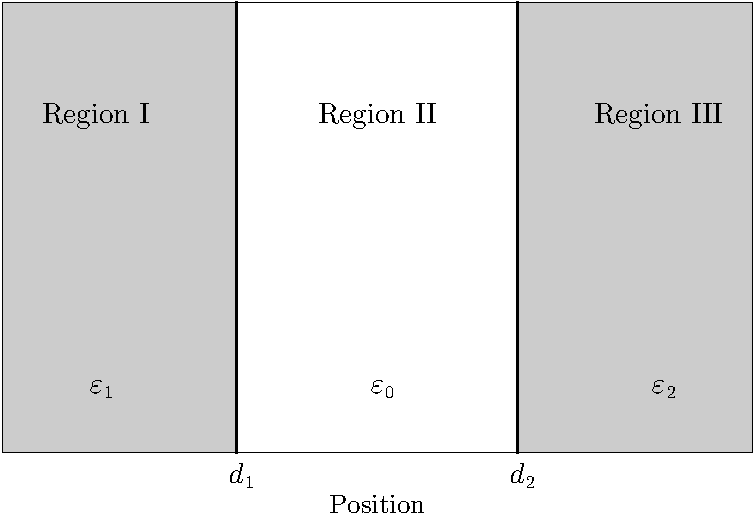
\includegraphics[width=0.6\linewidth]{fig/analytical/twoslab_ch3}
  \caption[Sketch of two planar dielectric slabs]{
    Sketch of two planar dielectric slabs, with dielectrics $\epsilon_1$ and $\epsilon_2$, with interfaces at $x=d_1$ and $x=d_2$.
    The slabs are separated by vacuum.}
\end{figure}

The solutions all involve $1-r\supTE_1r\supTE_2e^{-2\sqrt{2\lambda}d}$ in the denominators.
This factor was previously encountered in deriving the Lifshitz formula in Sec.~\ref{sec:lifshitz},
so it's presence is perhaps not surprising. 
However, in this case there is no need to make any conditions on which modes contribute.  
In addition, this derivation assumes there is vacuum between the dielectrics, although it could be easily generalized.

We will not attempt to invert the Laplace transform to find the solution in the time domain.
Later we will convert the worldline energy into a suitable form to use these results as written.  
However, in the strong coupling ($r\supTE_i\rightarrow -1$) limit, 
the Laplace transform can be inverted. In that case the denominator can be expanded by using
$(1-e^{-2\sqrt{2\lambda}d})^{-1}=\sum_{n}(-1)^n e^{-2n\sqrt{2\lambda}d}$ since $e^{-2\sqrt{2\lambda}d}<1$.  
The $n^{\text{th}}$ order term corresponds to the $n^\text{th}$ reflection
from the far surface.
After inverting the Laplace transforms, each Gaussian in the sum would be of the form $\exp[-2(n+1)^2d^2/t]$, corresponding
to the probability for a Brownian path to bounce $n$ times between points a distance $d$ apart.
This naturally goes over to the reflection picture for the Dirichlet scalar discussed in \S21.1.5.3 of Steck~\cite{SteckNotes}.

\section{Feynman--Kac Formula for Singular Potentials}
\label{sec:TM_potential}
The same methods can be used to yield sensible, finite results for worldline path integrals
involving singular potentials, such as $V\subTE$ and $V\subTM$ where
\begin{equation}
  V\subTM(x) = \frac{1}{2}\big[(\partial_x\log\sqrt{\epsilon})^2-\partial_x^2\log\sqrt{\epsilon}\big].
\end{equation}
(We will focus on $V\subTM$, since $\mur=1$ for almost all materials, so $V\subTE=0$.)
For a dielectric with a step-function discontinuity $\epsr = 1+\chi\Theta(x-d)$, the resulting
potential is highly singular.  
The first derivative of a step-function is a $\delta$-function, and 
the second derivative is $\delta'$, or the derivative of a $\delta$-function.
 We define a parameter $\Xi:=\log\sqrt{1+\chi}$, which means
$\log\sqrt{\epsr}(x) = \Xi\theta(x-d)$.  If the derivatives are taken directly then the potential is given by
\begin{equation}
  V\subTM(x) \sim \frac{1}{2}\big[\Xi^2\delta^2(x-d)-\Xi \delta'(x-d)\big],
\end{equation}
which involves the square of the $\delta$-function!  
The only way to make sense of this is to regularize the singularity in the step-function,
and take the limit of vanishing regularization at the end of the computation. 

We will consider an exponential interpolation of the dielectric between the two values $1$ and $1+\chi$,
over a distance $a$,
\begin{equation}
  \epsr\supa(x)= \left\{\begin{array}{ccr} 
      1 & \hspace{0.5cm} &x<d\\ 
      e^{2\Xi (x-d)/a} & \hspace{0.5cm}&d<x<d+a\\
      1+\chi & \hspace{0.5cm}&x>d+a
    \end{array}.
  \right.\label{eq:eps_reg}
\end{equation}
% \begin{equation}
%   \epsr\supa(x)= \Theta(d-x) + \Theta(x-d)\Theta(d+a-x)e^{2\Xi (x-d)/a} + \Theta(x-d-a)(1+\chi)
%   %     1 & \hspace{0.5cm} &x<d\\ 
%   %     e^{2\Xi (x-d)/a} & \hspace{0.5cm}&d<x<d+a\\
%   %     1+\chi & \hspace{0.5cm}&x>d+a
%   %   \end{array}.
%   % \right.
% \end{equation}
The logarithm of the dielectric can then be written
\begin{equation}
  \log\sqrt{\epsr\supa}(x)  
= \left\{\begin{array}{ccr} 
      0 & \hspace{0.5cm} &x<d\\ 
      \frac{\Xi}{a}(x-d)& \hspace{0.5cm}&d<x<d+a\\
      \Xi & \hspace{0.5cm}&x>d+a
    \end{array}.
  \right.
\end{equation}
The regularized TM potential is now given by 
\begin{equation}
  V\subTM\supa(x) = \frac{\Xi^2}{2a^2}\Theta(x-d)\Theta(d+a-x)-\frac{\Xi}{a}[\delta(x-d)-\delta(x-d-a)\big],
  \label{eq:VTM_reg}
\end{equation}
and is sketched in Fig.~\ref{fig:TMpot}.
The worst singularities present are the $\delta$-functions from the second derivative.
Although the potential is still singular, and cannot be handled nicely for just a single path, the ensemble
averaged expression over many such paths is well behaved. 

\begin{figure}
  \centering
  \includegraphics[width=0.4\linewidth,angle=90]{fig/analytical/TMpot}
  \caption[Regularized TM Potential]{Schematic drawing of a regularized TM potential~(\ref{eq:VTM_reg})
    at a regularized dielectric surface~(\ref{eq:eps_reg}). 
    Vertical arrows denote $\delta$-functions with heights $\Xi/a$, and solid rectangle marks the 
    step function of height $(\Xi/a)^2$.  }
  \label{fig:TMpot}
\end{figure}


\subsection{Transfer Layer Boundary Conditions for the TM Potential}

We will show that the regularized TM potential imposes an effective boundary condition at the interface. 
The diffusion equation can be solved inside the boundary layer $x\in(d,d+a)$, and all references 
to the interior can be eliminated.  The result of this will be conditions relating
the solution and its derivatives on either side of the surface.
Points starting inside the surface will not be considered, since the surface is infinitesimally thin.

The analytical solutions for the path integral obey
\begin{equation}
  \frac{1}{2}\partial_x^2f =\bigg(\lambda+\frac{\Xi^2}{2a^2}\Theta(x-d)\Theta(d+a-x)
  - \frac{\Xi}{2a}[\delta(x-d)-\delta(x-d-a)]\bigg)f
\end{equation}
Since $a$ is small, $\Xi/a$ is large relative to $\lambda$, so $\lambda$ which can be ignored in the thin-surface limit.    
At $x=d$, and $x=d+a$, $\delta$-function boundary conditions~(\ref{eq:delta_BC}) will be enforced.

Let $f_{\text{mid}}$ be the solution in the middle region for $x\in(d,d+a)$,   
    \begin{align}
      f_{\text{mid}} %=& Be^{\sqrt{2\lambda + \Xi^2/a^2}x} + C e^{-\sqrt{2\lambda + \Xi^2/a^2}x}\\
      =& Be^{\Xi x/a} + C e^{-\Xi x/a},
    \end{align}
    where $B$ and $C$ are constants to be determined.
%    Our goal is to derive the effective conditions imposed on the solutions just outside the surface.
    Let the solutions from the left be $f_1:=f(d-0_+)$, and the gradient $\partial_x f_1:=\partial_x f(d-0_+)$,
    with corresponding solutions on the right $f_2:=f(d+a+0_+)$, $\partial_x f_2:=f(d+a+0_+)$.  As far as this 
    calculation is concerned, these left and right solutions are unspecified constants. 
    The continuity conditions at $x=d$ and $x=d+a$ require that
    \begin{subequations}
      \begin{align}
        f_{\text{mid}}(d)-f_1 &= 0 \label{eq:f1}\\
        f_2- f_{\text{mid}}(d+a)&= 0 \label{eq:f2}\\
        \partial_xf_{\text{mid}}(d) -\partial_xf_1&= -\frac{\Xi}{a} f_1\label{eq:f1'}\\
        \partial_x f_2 -\partial_x f_{\text{mid}}(d+a)&= +\frac{\Xi}{a} f_2.\label{eq:f2'}
      \end{align}
    \end{subequations}
   These equations can be solved for the internal parameters $B$ and $C$, as well as two of the external 
   parameters, $f_2$ and $\partial_x f_2$ in terms of $f_1$ and $\partial_x f_1$.
   As a result, we will have found simple effective boundary conditions between
   the field values $f_1,\partial_xf_1$ and $f_2,\partial_xf_2$ on either side of the boundary.
%   Given this calculation's importance to our subsequent work, we will actually go through the elementary algebra.  

   % Find relations between $f(d\pm \epsilon)$ and $f'(d\pm \epsilon)$.
   %  We will solve for $f(d+a+\epsilon)$, and $f'(d+a+\epsilon)$,
   %  trying to eliminate $B$ and $C$, which we will fix in terms of $f(d-\epsilon),f'(d-\epsilon)$.
   %  We will thus have derived the relation between $f$ and its derivatives on both sides of the potential.      
    The continuity conditions in Eqs.~(\ref{eq:f1}) and (\ref{eq:f2}) require that
    \begin{align}
      f_1 &= Be^{\Xi d/a} + C e^{-\Xi d/a}\label{eq:M c1}\\
      f_2 &= Be^{\Xi d/a+\Xi} + C e^{-\Xi d/a-\Xi}\label{eq:M c2}.
    \end{align}
    The derivative conditions in Eqs.~(\ref{eq:f1'}) and (\ref{eq:f2'}) then require that
    \begin{align}
      \partial_xf_1&= 2\frac{\Xi}{a}Be^{\Xi d/a} \label{eq:M d1}\\
      \partial_xf_2&=2\frac{\Xi}{a}Be^{\Xi d/a}e^{\Xi}\label{eq:M d2},
    \end{align}
    where the continuity conditions have been exploited.
    From the derivative conditions, $\partial_xf_1$ and $\partial_xf_2$ can be related to one another:
%    Eq.~(\ref{eq:M d1}) fixes $B$, which we can use in to Eq.~(\ref{eq:M d2}), so that 
    \begin{equation}
      \partial_xf_2 = e^{\Xi}\partial_xf_1.
    \end{equation}
    In addition, under the assumption that the external gradients $\partial_x f_1$, $\partial_xf_2$ are independent of $a$ and order one,
    that also implies that $B\sim\order(a)$, since $\frac{B}{a}$ must be finite.  
    That implies that in the continuity conditions $B$ is much smaller than $C$ which must also be order one.
    On setting $B=0$, it is clear from Eqs.~(\ref{eq:M c1})-(\ref{eq:M c2}) that 
    \begin{equation}
      f_2 =  e^{-\Xi} f_1.  
    \end{equation}
    At this point, the conditions between the solutions outside the boundary layer have been derived,
    and the  $a\rightarrow 0$ limit can be taken everywhere.  
    The regularized dielectric step produces the following effective boundary boundary conditions at an interface
    \begin{align}
      \Aboxed{
        f(d+0_+) =& e^{-\Xi}f(d-0_+) \qquad
        \partial_xf(d+0_+)= e^{\Xi}\partial_xf(d-0_+)
      }\label{eq:TM_boundary_conditions}
    \end{align}
    \label{sec:TM boundary condition}
    These boundary conditions can then be used to find the ensemble average solution for the 
    regularized TM potential.  

\subsection{Finding the Path Integral Solution for the TM Potential}

% We can now find the Feynman--Kac formula for open Brownian bridges near a single TM-potential, which 
% imposes the boundary conditions~\ref{eq:TM_boundary_conditions}.  This solution is the ensemble average 
% over all Brownian paths between the end points.

We aim to find a closed form solution for the path integral over paths between starting at $x=0$ and terminating at $c$ after time $t$ and 
interacting with potential $V\subTM$,
\begin{equation}
  f\subTM(c,d,\Xi)=\int_0^\infty dt\, e^{-\lambda t}\frac{e^{-c^2/(2t)}}{\sqrt{2\pi t}} \dlangle e^{-\int_0^T dt\, V_{TM}}\drangle.
\end{equation}
The Gaussian factor is the normalization for a 1D Brownian bridge between $x=0$ and $c$ in time $t$.
This path integral is found by solving
\begin{equation}
  0 = \frac{1}{2} \partial_x^2 f\subTM - (V\subTM+\lambda)f\subTM + \delta(x-c),
\end{equation}
where TM boundary conditions~(\ref{eq:TM_boundary_conditions}) are imposed at $x=d$,
and $\delta$-function boundary conditions~(\ref{eq:delta_BC}) are imposed at $x=c$.  
The solutions naturally decompose into two cases: first,  when the end points of the path are on the same
side of the surface,  and when they are on different sides.
% \comment{    Note how to recover various cases by flipping signs etc.  
%     Simplify down to crossing/no-crossing cases.}
%    That seems complicated, but we can note that if there is a crossing ($|c|<|d|$) then we get 
    When both points are on the same side, or $d(d-c)>0$, the solution is 
    \begin{equation}
      f\subTM=\dfrac{e^{-\sqrt{2\lambda}|c|}}{\sqrt{2\lambda}} 
      + \sgn(d)\dfrac{e^{-\sqrt{2\lambda}|2d-c|}}{\sqrt{2\lambda}}\dfrac{e^{2\Xi}-1}{e^{2\Xi} +1},
    \end{equation}
    where $\sgn(x)$ is the signum function: $\sgn(0)=0$, $\sgn(x>0)=1$, $\sgn(x<0)=-1$.
    When the paths must cross through the surface since $x=0$ and $c$ are on different sides of the surface so $d(d-c)<0$,
    the solution is
    \begin{equation}
      f\subTM = \dfrac{ e^{-\sqrt{2\lambda}|c|}}{\sqrt{2\lambda}} \dfrac{2e^\Xi}{1 + e^{2\Xi}}.
    \end{equation}
      The material constants can be rewritten in terms of $\chi$, by using $\Xi=\log\sqrt{1+\chi}$,
      with the result
      \begin{align}
        \tanh\Xi &=\dfrac{e^{2\Xi}-1}{e^{2\Xi} +1} =\dfrac{\chi}{2+\chi}=\frac{\epsilon_{\text{r},1} -1}{\epsilon_{\text{r},1}+1}\\
        \sech\Xi &= \dfrac{2e^\Xi}{1 + e^{2\Xi}} = \frac{2\sqrt{1+\chi}}{2+\chi}.
      \end{align}
    In both cases the Laplace transforms in $\lambda$ can be inverted yielding Gaussians [following from Eq.~(\ref{eq:Laplace_Gaussian})].
    After canceling out the Gaussian factor $e^{-c^2/(2t)}/\sqrt{2\pi t}$, the analytical expression for 
    the path integral can be isolated
    % Ultimately, we will want to isolate the potential term.  
    % If we use 
    % \begin{equation}
    %   \mathcal{L}^{-1}\left[ \frac{e^{-\sqrt{2\lambda}x}}{\sqrt{2\lambda}}   \right] = \frac{e^{-x^2/(2t)}}{\sqrt{2\pi t}},
    % \end{equation}
    % which is exactly the factor we isolated in front of $\mathcal{M}$.  
    \begin{align}
      \dlangle e^{-\int_0^t dt'\, V\subTM(x-d)}\drangle 
      &=\left\{ \begin{array}{lc} 
          1   + \sgn(d)\tanh\Xi\, e^{-2d(d-c)/t} & d(d-c)>0\\
          \sech\Xi & d(d-c)<0
        \end{array}
        \right.  \label{eq:TM_potential}
      \end{align}
      This result is absolutely crucial for developing numerical methods for the TM polarization.  
      Even the regularized potential is too unruly to handle on a single trajectory wise basis.  The analytical
      solution smooths the result out by averaging over all possible sub-paths. 
      The result can be extended to include any starting point $x_i$ by shifting $d\rightarrow d-x_i$,
      and identifying $c=x_f-x_i$, where $x_f$ is the final point.


    \begin{figure}
      \centering
      \includegraphics[width=0.8\linewidth]{fig/analytical/TMsoln}
      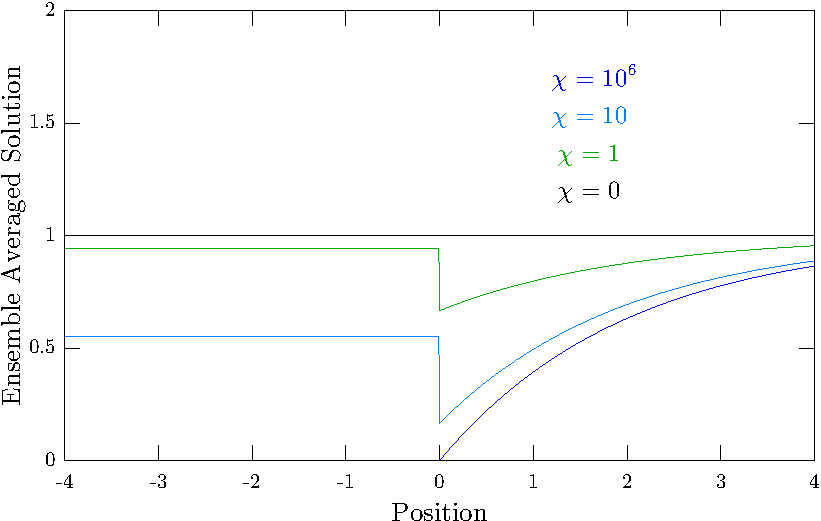
\includegraphics[width=0.8\linewidth]{fig/analytical/TMsoln2}
      \caption[Plot of TM Solution]{
        Plot of ensemble-average TM solution~(\ref{eq:TM_potential}) 
        outside dielectric step at the origin$\epsr=1+\chi\theta(x)$ for various various $\chi$,
        as function of final position $x$.
        Top plot considers paths starting outside medium at $x_0=-1$, while lower plot considers paths
        starting inside the medium at $x_0=1$.
      }
      \label{fig:TM_plot}
    \end{figure}



      The potential has been plotted in Fig.~\ref{fig:TM_plot} as a function of ending point
      for paths starting inside and outside the barrier.  
      Note that the potential leads to larger values on the vacuum side of the medium, 
      and suppresses values for starting points inside the surface or paths that must cross the surface.  

      In the strong-coupling limit $\tanh\Xi\rightarrow 1, \sech\Xi\rightarrow 0$, and the solution for 
      paths starting at the origin is
    \begin{align}
      f_N      &=\theta[d(d-c)]\bigg( 1 +\sgn(d)\dfrac{e^{-2d(d-c)/t}}{\sqrt{2\pi t}}\bigg).
      \end{align}
      This is in some sense dual to the Dirichlet limit.  In that case paths reflect off with the opposite phase, 
      leading to a value of zero on the boundary.  Here, the paths reflecting off the surface add in phase, suggesting 
      a correspondence to Neumann boundary conditions.  However, this does not hold for paths starting 
      inside the surface, where the solution is the same as for Dirichlet boundary conditions.  
    

    % Dan has:
    % \begin{equation}
    %   \dlangle \exp\left[-\int_0^T dt V_{TM}(x-d)\right]\drangle = 1 + \frac{\sinh(\Xi/2)}{\cosh\Xi}[\sgn(d-c)e^{\sgn(d)\Xi/2} + \sgn(d)e^{-\sgn(d)\Xi/2}]e^{\left[c^2-(|d|+|c-d|)^2\right]/2t}.
    % \end{equation}
    % This agrees with my expressions for all cases.  This is useful for our numerical work.  
    % Let us check out the $\Xi$ prefactor against my work.  
    % \begin{align}
    %   F_{d>0,c<d} =&\frac{\sinh(\Xi/2)}{\cosh\Xi}[\sgn(d-c)e^{\sgn(d)\Xi/2} + \sgn(d)e^{-\sgn(d)\Xi/2}]\\
    %   =&\frac{\sinh(\Xi/2)}{\cosh\Xi}[e^{\Xi/2} + e^{-\Xi/2}] = \frac{e^{\Xi} - e^{-\Xi}}{e^\Xi+ e^\Xi}  
    % \end{align}
    % works.
    % \begin{align}
    %   F_{d>0,d<c} =&\frac{\sinh(\Xi/2)}{\cosh\Xi}[-e^{\Xi/2} + e^{-\Xi/2}] = -\frac{ e^{-\Xi} + e^{\Xi} -2}{e^\Xi + e^{-\Xi}},
    % \end{align}
    % works, 
    % \begin{align}
    %   F_{d<0,c<d} =\frac{\sinh(\Xi/2)}{\cosh\Xi}[e^{-\Xi/2} -e^{\Xi/2}]=\frac{[(e^{\Xi/2}- e^{-\Xi/2})(e^{-\Xi/2} -e^{\Xi/2})]}{e^\Xi + e^{-\Xi}}=-\frac{e^\Xi + e^{-\Xi} -2}{e^\Xi + e^{-\Xi}},
    % \end{align}
    % works, and 
    % \begin{align}
    %   F_{d<0,d<c} =&\frac{\sinh(\Xi/2)}{\cosh\Xi}[-e^{\Xi/2} -e^{-\Xi/2}] = -\frac{e^\Xi - e^{-\Xi}}{e^\Xi + e^{-\Xi}}
    % \end{align}

\section{Single TM potential and Step}

Next, we consider a dielectric step combined with a TM boundary condition.  
This is required to analytically compute the TM component of the Casimir--Polder energy for an atom near a
dielectric half-space.  We will only develop the solution for closed paths.
The path integral
    \begin{equation}
      f = \int_0^\infty dt\, e^{-\lambda t}\frac{1}{\sqrt{2\pi t}}\bigdlangle e^{-\int_0^t dt'\, [V\subTM(x,d) + \chi\Theta(x-d)]}\bigdrangle ,
    \end{equation}
    is the steady-state solution to 
    \begin{equation}
      \partial_t f = \frac{1}{2}\partial_x^2f -[V_{TM}(x,d) + \chi\Theta(x-d)+\lambda]f +\delta(x). 
    \end{equation}
    The analytical expression is found by solving the diffusion equation directly, with 
    TM boundary conditions~(\ref{eq:TM_boundary_conditions}) at $x=d$ and 
    $\delta$-function boundary conditions~(\ref{eq:delta_BC}) at $x=0$.
    The solution for a single TM body is 
  \begin{equation}
      f_{TM,1}(x) = \left\{\begin{array}{lcr} 
          \dfrac{1}{\sqrt{2\lambda}}\left(1+ r\supTM e^{-2\sqrt{2\lambda}d}\right)  & \hspace{2cm} & d<0\\
          \dfrac{1}{\sqrt{2(\lambda+\chi)}}\left(1 - r\supTM e^{-2\sqrt{2(\lambda+\chi)}d}\right) & \hspace{2cm} & d>0\\
        \end{array} \right. 
      \label{eq:Feynman-Kac TM one step}
    \end{equation}
    where
    \begin{equation}
      r\supTM = \frac{\sqrt{\lambda}e^{2\Xi} -\sqrt{\lambda+\chi}}{\sqrt{\lambda}e^{2\Xi} + \sqrt{\lambda+\chi}}.
      \label{eq:TM_coeff}
    \end{equation}
    The reflection coefficient $r\supTM$ corresponds to the TM reflection coefficient 
    used in Sec.~\ref{sec:lifshitz}, since $e^{2\Xi}=1+\chi$.  
    This calculation can also be naturally extended to include a magnetic response, since $\Xi$ and $\chi$
    can be treated as independent parameters.  
    The parameter $\Xi$ is defined in relation to the boundary condition, while $\chi$ relates to the 
    step discontinuity.  To describe the TM potential, one could take $\chi\rightarrow (\epsr\mur-1)$
    and $\Xi$ is unchanged.  Similar reasoning could apply these results to the TE potential,
    after the $\epsr\leftrightarrow \mur$ substitution is carried out.

    % Ultimately, we find that 
    % \begin{align}
    %   &\int_0^\infty dT e^{-\lambda T} \dlangle \frac{1}{\sqrt{2\pi T}}
    %   \exp\left(-\int_0^T dt \{V\subTM[x(t)]+s\theta[x(t)-d]\}\right)\drangle\nonumber\\
    %   &\hspace{1cm}=
    %   \frac{1}{\sqrt{2[\lambda+\chi\theta(d)]}}\left[1 - \sgn(d) r\supTM e^{-2\sqrt{2[\lambda+\chi\theta(d)]}|d|}\right]
    %   ,\label{eq:Feynman--Kac TM one step}
    % \end{align}
    % where the ensemble average is over brownian bridges that satisfy $x(0)=x(T)=0$.
    % The factor of $\sqrt{2\pi T}$ is normalization for the use of the bridges.  


\section{Two TM Step Potentials}

The preceding calculations for can be easily to handle two planar dielectric half-spaces subject to 
TM boundary conditions.  This time, the solution is  the path integral for a potential
\begin{equation}
  V = \chi_1\Theta(-d/2-x)+\chi_2\Theta(x-d/2)+V\subTM(-\Xi_1,d_1)+V\subTM(\Xi_2,d_2)
\end{equation}
In this case a little care is needed in defined the boundary conditions at the left hand surface.
Since the left body has the opposite orientation (the permittivity decreases as $x$ increases at $x=-d/2$)
the correct TM potential for the left body has $\Xi_1\rightarrow-\Xi_1$ everywhere.
This change reverses the nature of the effective boundary conditions at the surface: if passing 
through the surface decreases the function, and increases the gradient, then traversing the surface in the   
opposite direction should have the opposite effect.  So at the left hand-surface, the boundary conditions 
are 
    \begin{align}
        f(d_1+0_+) =& e^{\Xi_1}f(d_1-0_+) \qquad      \partial_xf(d_1+0_+)= e^{-\Xi_1}\partial_xf(d_1-0_+).
    \end{align}


The resulting solutions have the same form and structure as the TE solutions, but with 
the TE reflection coefficients replaced by their TM counterparts.  
% (This simple correspondence was not anticipated given the highly singular form of the TM potentials.  
% Only the regularization, and the analytical averaging over sub-paths allowed this simplicity to emerge.)
The two-body TM solution can be written in the same three regions as two-body TE solution:%  where 
% For paths starting in the left body, $x_0<d_1$ the solution is
\begin{subequations}
    \label{eq:Feynman-Kac TM two step}
    \begin{align}
      f^{(\text{I})}\subTMtwo(x) &=
           \dfrac{1}{\sqrt{2(\lambda+\chi_1)}} + e^{-2\sqrt{2(\lambda+\chi_1)}(d_1-x_0)}
 \dfrac{r\supTM_2 e^{-2\sqrt{2\lambda}d} - r\supTM_1}{\sqrt{2(\lambda+\chi_1)}(1-r\supTM_1r\supTM_2 e^{-2\sqrt{2\lambda}d})}\\
      f^{(\text{II})}\subTMtwo(x)&= %= \frac{1}{\sqrt{2\lambda}} + \frac{2r\supTM_1r\supTM_2 e^{-2\sqrt{2\lambda}d} + r\supTM_1 e^{2\sqrt{2\lambda}h} +r\supTM_2 e^{-2\sqrt{2\lambda}(d+h)}}{\sqrt{2\lambda}(1-r\supTM_1r\supTM_2 e^{-2\sqrt{2\lambda}d})}
          \frac{1}{\sqrt{2\lambda}} + 
          \dfrac{2r\supTM_1r\supTM_2 e^{-2\sqrt{2\lambda}d} + r\supTM_1 e^{2\sqrt{2\lambda}(d_1-x_0)} +r\supTM_2 e^{-2\sqrt{2\lambda}(d_2-x_0)}}
          {\sqrt{2\lambda}(1-r\supTM_1r\supTM_2 e^{-2\sqrt{2\lambda}d})}\\
            f^{(\text{III})}\subTMtwo(x)&= %=  \frac{1}{\sqrt{2(\lambda+\chi_2)}} + \frac{e^{2\sqrt{2(\lambda+\chi_2)}(d+h)}(r\supTM_1 e^{-2\sqrt{2\lambda}d} - r\supTM_2)}{\sqrt{2(\lambda+\chi_2)}(1-r\supTM_1r\supTM_2 e^{-2\sqrt{2\lambda}d})},
          \dfrac{1}{\sqrt{2(\lambda+\chi_2)}} + e^{2\sqrt{2(\lambda+\chi_2)}(d_2-x_0)}
          \dfrac{(r\supTM_1 e^{-2\sqrt{2\lambda}d}-r\supTM_2)}{\sqrt{2(\lambda+\chi_2)}(1-r\supTM_1r\supTM_2 e^{-2\sqrt{2\lambda}d})},
    \end{align}
  \end{subequations}
  where the TM reflection coefficients for each body are given by 
    \begin{equation}
      r\supTM_i = \frac{e^{2\Xi_i}\sqrt{\lambda} -\sqrt{\lambda+\chi_i}}{e^{2\Xi_i}\sqrt{\lambda} + \sqrt{\lambda+\chi_i}}.
      \label{eq:uTM_i}
    \end{equation}
  % \item {Integrate over position}
%     In exactly the same fashion, we can integrate over position.  
%     \begin{align}
%       I_{TM,12} =& -I_{div} + \dfrac{r\supTM_2 e^{-2\sqrt{2\lambda}d}-r\supTM_1}{4(\lambda+\chi_1)(1-r\supTM_1r\supTM_2 e^{-2\sqrt{2\lambda}d})} +\frac{2r\supTM_1r\supTM_2 e^{-\sqrt{2\lambda}d}d}{\sqrt{2\lambda}(1-r\supTM_1r\supTM_2 e^{-2\sqrt{2\lambda}d})} + (r\supTM_1+r\supTM_2)\frac{(1-e^{-2\sqrt{2\lambda}d})}{4\lambda(1-r\supTM_1r\supTM_2e^{-2\sqrt{2\lambda}d})}\nonumber\\
%       & +\frac{r\supTM_1 e^{-2\sqrt{2\lambda}d} - r\supTM_2}{4(\lambda+\chi_2)(1-r\supTM_1r\supTM_2 e^{-2\sqrt{2\lambda}d})},
%     \end{align}
%     where $I_{div} = [2(\lambda+\chi_1)]^{-1/2}\int_{-\infty}^h dx_0  +  [2(\lambda+\chi_2)]^{-1/2}\int_{h+d}^\infty dx_0  + (2\lambda)^{-1/2}d$.
%   \item Comment on divergent parts cancelling out. 
% \end{enumerate}
This result contains all of the previous results for closed paths.  
The TE results are recovered by taking $\Xi\rightarrow 0$.
In taking $\chi\rightarrow 0$, the dielectric steps can be ignored, and this is the two body result for just the TM
boundary conditions.  
The equivalent single body results can be found by taking the far body to $x=\pm\infty$.  

These formulae are most useful for showing the analytical agreement with existing 
Casimir energy results.  As such it is best to leave them in this Laplace-transformed form.  
The next chapter uses the results from this chapter to re-derive known analytical results for both 
polarizations for Casimir and Casimir--Polder energies.  

%%% Local Variables: 
%%% mode: latex
%%% TeX-master: "thesis_master"
%%% End: 
